\chapter{Design}

\section{Architecture}

The designed architecture of the project can be observed in the figure \ref{fig:arch}. There are three data sources connected to Grafana through an extended version of the official SimpleJson data source plugin. Each data source access the data it provides in different ways; through an outside service, from a database or from memory.

\begin{figure}[h]
	\centering
	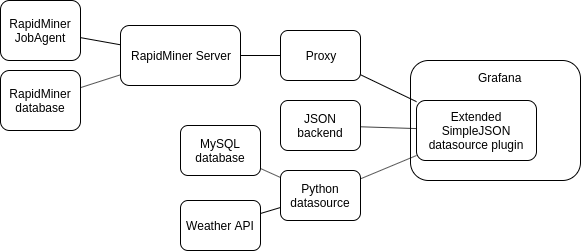
\includegraphics[width=150mm, keepaspectratio]{figures/architecture.png}
	\caption{Architecture diagram}
	\label{fig:arch}
\end{figure}

%---
\section{Components}
%---

In this section, each component is presented, focusing on their responsibilities.

%---
\subsection{Extended SimpleJSON datasource plugin}
%---

Grafana uses data source plugins to connect to different data storage backends. Each data source plugin exposes a Grafana specific interface which allows Grafana to communicate with each data source plugin the same way.

% https://github.com/grafana/simple-json-datasource
The SimpleJSON datasource is made by the Grafana team and is available on GitHub (insert reference HERE).

It has two main purposes. One is to act as an example implementation to make writing custom data source plugins easier for the community. The other is to enable Grafana to read data from services that expose data in JSON format (which is widely popular thorough the industry).

For this thesis project, the latter role seems to be more important, as it possible to create a tool that receives data from different kind of formats and translates them into JSON. This way, we can send the transformed data to Grafana, which as a result would be able to display the collected data in one place that originally came from various sources.

In order to introduce additional interactivity capabilities, when integrating the RapidMiner Webservice, the SimpleJSON data source plugin needs to be extended. 

\begin{center}
	--- TODO ---
	\begin{itemize}
		\item extended API for SimpleJSON datasource
		\subitem querying available paramaters for a RM webservice
	\end{itemize}
\end{center}


%---
\subsection{Proxy}
%---

The main responsibility of this component is to translate between the RapidMiner Web service which the RapidMiner Server exposes and the SimpleJSON datasource plugin. The problem is that RapidMiner Server exposes its result in JSON, but is in another format that the SimpleJSON datasource plugin accepts.

%---
\subsection{JSON backend}
%---
% https://github.com/bergquist/fake-simple-json-datasource
This component is a example backend implementation for the SimpleJSON data source plugin. It serves as a base for creating other backends for the data source plugin. It also further expresses the general usability of the SimpleJSON plugin.

%---
\subsection{Python data source}
%---

\begin{center}
	--- TODO ---
\end{center}


%---
\subsection{Weather API}
%---

This component represents the previously mentioned external service. Its responsibility is to expose a service that can be utilized by other softwares in order to acquire additional business-relevant information.

%---
\subsection{MySQL database}
%---

The Python datasource uses this database component to read some sample data from it.


%\begin{itemize}
%	\item why do we need a gateway
%	\item how can we access data from RapidMiner WebService
%	\item why is it good to have a python compoment between Grafana and MySQL
%	\begin{itemize}
%		\item we can customize it better, what we see from the database
%		\item can implement business logic, only see business-relevant projections, granularity of the data
%		\item can aggregate data from different backends
%		\item can aggregate data with outsider APIs (POC implementation for this use-case)
%	\end{itemize}
%\end{itemize}


\begin{itemize}
	\item Grafana
	\item proxy/gateway
	\item python-datasource
	\begin{itemize}
		\item python-datasource
		\item mysql
		\item weather-api
	\end{itemize}
	\item RapidMiner stack
	\begin{itemize}
		\item rapidminer-server
		\item job-agent
		\item database
	\end{itemize}
	\item Grafana datasource plugin (extended API - parameters)
	\begin{itemize}
		\item extended API for asking for available parameters
		\item extended GUI, that dynamically lists available parameters (specify SOURCE!!!!!!!)
	\end{itemize}
	\item Grafana extended panel plugin
\end{itemize}